% Provenance (never printed): old seconde/premiere S material on soil as a
% slowly renewed resource (alteration of rocks, clays, the clay--humus
% complex, soil erosion); see sources/book2/PROVENANCE.md. Rates are the
% medians of Montgomery (2007), computed in figdata/grade-10/soil_rates.py.
\chapter{Tanah, Sumber Daya yang Lambat Terbentuk}\label{ch:g10:soil-formation}

Sebuah potongan jalan yang membelah lereng bukit di daerah tropis basah
memperlihatkan dinding tanah merah, beberapa kali tinggi orang. Di kakinya
batuan masih dapat dikenali: pucat, bergaris-garis, tetapi begitu lunak
sehingga hancur di antara jari-jari sambil masih memperlihatkan butir-butir dan
pita-pita batuan asalnya. Makin ke atas batuan itu berubah menjadi lempung
berbercak, lalu menjadi lapisan merah yang keras, lalu menjadi tanah tipis
tempat akar-akar berada. Seluruh dinding itu dahulu adalah batuan padat:
dinding itu adalah batuan itu sendiri, yang perlahan-lahan diubah di tempatnya
oleh air dan udara. Tanah, tempat tumbuhnya semua tumbuhan di daratan dan
makanan hampir semua manusia, adalah bagian atas kolom seperti itu. Bab ini
menjelaskan bagaimana batuan menjadi tanah, kimia apa yang melakukan
pekerjaan itu, bagaimana iklim menentukan lajunya, dan mengapa tanah, yang
begitu lambat terbentuk, dapat hilang begitu cepat.

\begin{omfigure}
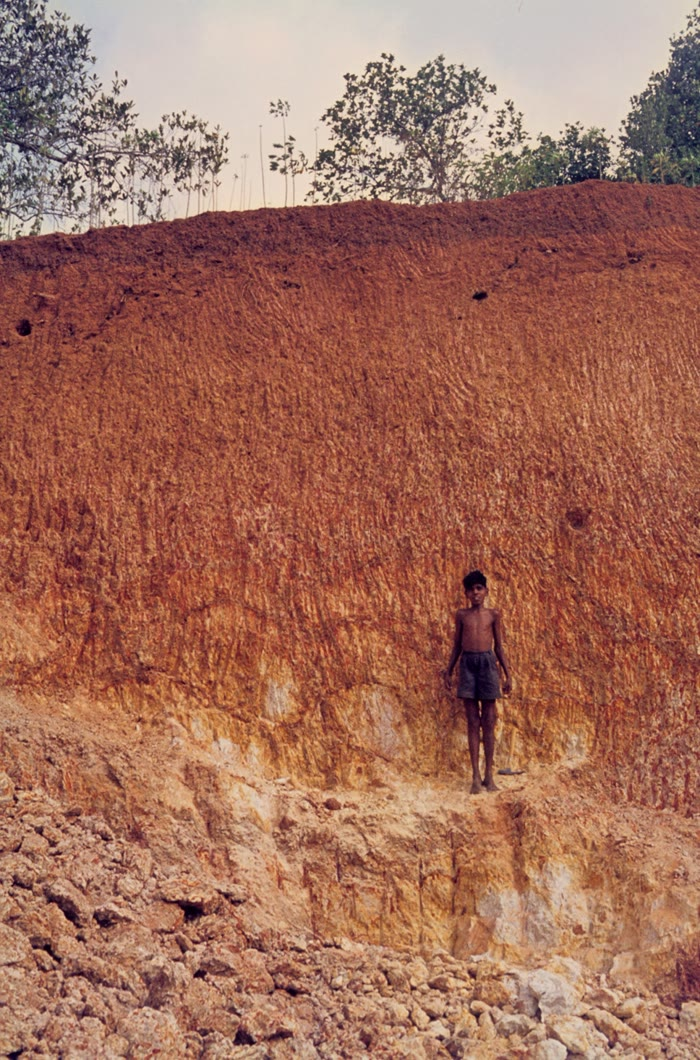
\includegraphics[height=8.5cm]{images/book2/g10-laterite-kerala.jpg}

{\small Profil pelapukan pada gneis granitik di Kerala, India selatan: di
bagian bawah, batuan yang terurai dan berbercak; di atasnya, \omterm{def:g10:soil-formation:laterite}{laterit} cokelat
yang sedikit mengeras di bawah tanah yang tipis. Anak laki-laki itu
menunjukkan skalanya. Foto: Werner Schellmann, 1969 (CC~BY-SA~2.5).}
\end{omfigure}

\begin{recall}
Pelapukan menghancurkan batuan di tempatnya; erosi mengangkut
pecahan-pecahannya; pengendapan meletakkannya di tempat lain (Buku 1, kelas
5). Batuan tersusun atas mineral, seperti kuarsa, feldspar, dan mika dalam
granit (Buku 1, kelas 6). Tanah adalah lapisan hidup yang terdiri atas
butir-butir mineral, humus, air, udara, dan organisme; pengurai mengubah
bahan mati menjadi humus; tanah diuraikan menurut lapisan-lapisannya, atau
horizon (buku-buku biologi). Dalam oksidasi, suatu zat kehilangan elektron,
sering kali dengan bergabung dengan oksigen (buku-buku kimia).
\end{recall}

\section{Dari batuan menjadi tanah}

Pelapukan fisika --- pembajian oleh es, pemanasan dan pendinginan, akar ---
memecah batuan menjadi kepingan tanpa mengubah mineral-mineralnya. \omterm{def:g10:soil-formation:chemical-weathering}{Pelapukan
kimia} mengubah mineral-mineral itu sendiri. Bersama-sama, dalam waktu yang
lama, keduanya mengubah bagian atas batuan padat menjadi selimut lepas yang
menebal ke arah bawah seiring pelapukan menggerogoti batuan di bawahnya.

\begin{definition}[Batuan induk; saprolit]\label{def:g10:soil-formation:weathering-profile}
Yang disebut \emph{batuan induk}\index{batuan induk} sebuah tanah adalah batuan
yang darinya bagian mineral tanah itu terbentuk. Yang disebut
\emph{saprolit}\index{saprolit} adalah batuan yang terurai di tempatnya oleh
pelapukan: lunak dan bersifat tanah, saprolit masih memperlihatkan butir-butir
dan struktur batuan induk. \emph{Profil pelapukan} adalah seluruh kolom dari
batuan segar, melalui saprolit, sampai ke tanah di bagian atas.
\end{definition}
% ledger: usgs:saprolite

\omterm{def:g10:soil-formation:weathering-profile}{Saprolit} dapat tebal. Di bawah perbukitan yang bergelombang di sepanjang sisi
timur Pegunungan Appalachia, di Amerika Serikat bagian timur, tebalnya
mencapai sekitar \qty{46}{m} (150 kaki) di beberapa tempat, meskipun tebalnya
sangat berbeda-beda dari tempat ke tempat; tanah hanyalah bagian atasnya.
% ledger: usgs:saprolite

\begin{omfigure}
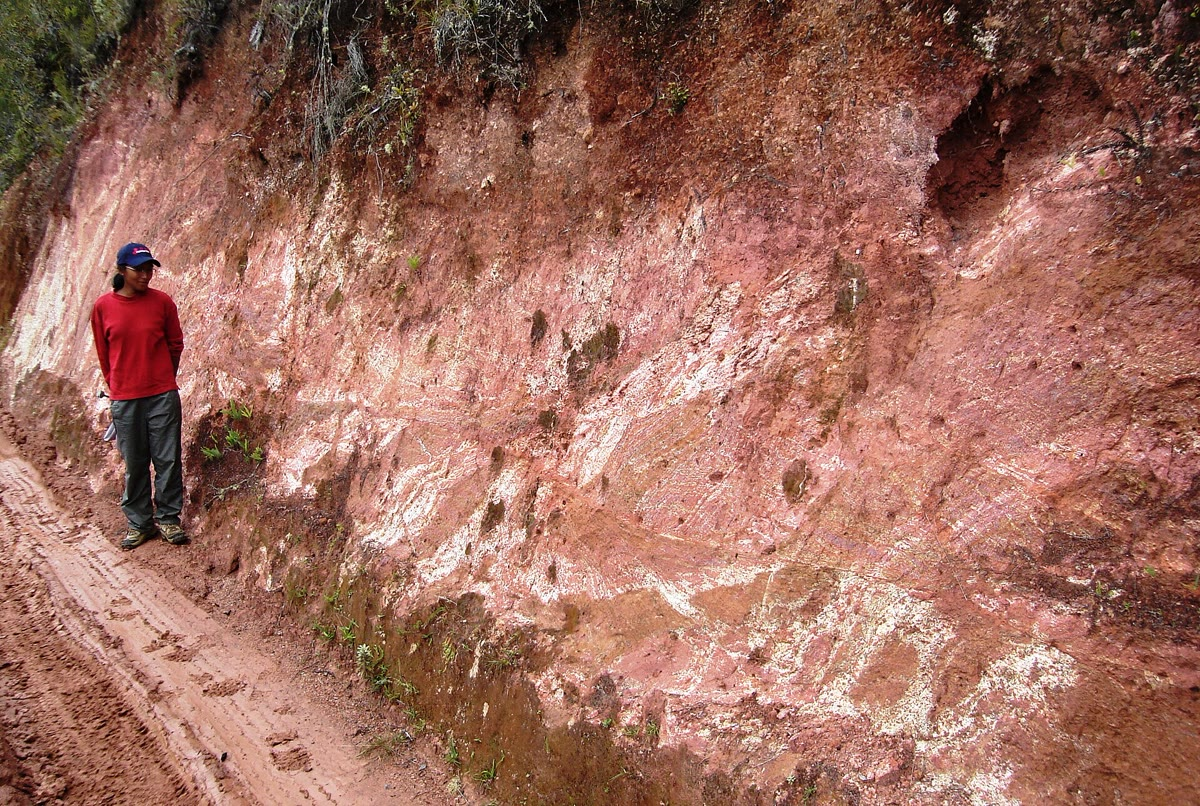
\includegraphics[width=0.8\linewidth]{images/book2/g10-saprolite-madagascar.jpg}

{\small \omterm{def:g10:soil-formation:weathering-profile}{Saprolit} di sebuah potongan jalan di Madagaskar tengah: gneis tua,
yang terurai di tempatnya, masih memperlihatkan pita-pitanya sebagai
garis-garis lempung putih dalam tanah merah. Foto: Diorit (CC~BY-SA~3.0).}
\end{omfigure}

\begin{omfigure}
\begin{tikzpicture}[font=\footnotesize]
  % humid tropical column
  \begin{scope}
    \fill[omThm!45!brown!60] (0,5.4) rectangle (1.8,6.0);
    \fill[omThm!70!orange!70] (0,4.2) rectangle (1.8,5.4);
    \fill[omThm!25!orange!35] (0,1.2) rectangle (1.8,4.2);
    \foreach \y in {1.5,2.1,2.7,3.3,3.9} \draw[white!80!black, thick] (0.1,\y) -- (1.7,\y+0.15);
    \fill[black!30] (0,0) rectangle (1.8,1.2);
    \foreach \x/\y in {0.3/0.3,0.9/0.7,1.4/0.2,0.5/0.9,1.2/1.0} \draw[black!55] (\x,\y) -- ++(0.2,0.08);
    \draw[black!60] (0,0) rectangle (1.8,6.0);
    \node[anchor=north, align=center] at (0.9,-0.1) {tropis basah};
  \end{scope}
  % temperate column
  \begin{scope}[xshift=3.2cm]
    \fill[omThm!45!brown!60] (0,2.2) rectangle (1.8,2.6);
    \fill[omThm!25!orange!35] (0,1.2) rectangle (1.8,2.2);
    \foreach \y in {1.5,1.9} \draw[white!80!black, thick] (0.1,\y) -- (1.7,\y+0.15);
    \fill[black!30] (0,0) rectangle (1.8,1.2);
    \foreach \x/\y in {0.3/0.3,0.9/0.7,1.4/0.2,0.5/0.9,1.2/1.0} \draw[black!55] (\x,\y) -- ++(0.2,0.08);
    \draw[black!60] (0,0) rectangle (1.8,2.6);
    \node[anchor=north, align=center] at (0.9,-0.1) {iklim\\sedang};
  \end{scope}
  % labels
  \draw[black!50] (5.3,5.7) -- (2.0,5.7); \node[anchor=west] at (5.4,5.7) {tanah};
  \draw[black!50] (5.3,4.8) -- (2.0,4.8); \node[anchor=west, align=left] at (5.4,4.8) {laterit: merah, kaya oksida\\besi dan aluminium};
  \draw[black!50] (5.3,3.4) -- (2.0,3.4); \node[anchor=west, align=left] at (5.4,3.4) {saprolit: batuan terurai\\di tempat, strukturnya tetap};
  \draw[black!50] (5.3,0.6) -- (5.0,0.6); \node[anchor=west] at (5.4,0.6) {batuan induk segar};
\end{tikzpicture}

{\small Dua profil pelapukan pada batuan yang sama (skematis, tidak
berskala): di bawah iklim yang panas dan basah profilnya jauh lebih tebal dan
bagian atasnya berupa \omterm{def:g10:soil-formation:laterite}{laterit}; di bawah iklim sedang \omterm{def:g10:soil-formation:weathering-profile}{saprolit} yang lebih tipis
menyangga tanah.}
\end{omfigure}

\section{Pelapukan kimia}

\begin{definition}[Pelapukan kimia]\label{def:g10:soil-formation:chemical-weathering}
Yang disebut \emph{pelapukan kimia}\index{pelapukan kimia} adalah perubahan
mineral-mineral batuan melalui reaksi dengan air dan dengan gas-gas yang
dibawanya, karbon dioksida dan oksigen: sebagian mineral melarut, sebagian
lain diubah menjadi mineral baru yang stabil di permukaan Bumi.
\end{definition}

Air hujan melarutkan sedikit karbon dioksida dari udara, dan jauh lebih banyak
ketika meresap melalui tanah, tempat akar dan pengurai mengembuskannya.
Sebagian gas terlarut itu membentuk asam karbonat, yang melepaskan ion
hidrogen:
\begin{center}
\ce{CO2 + H2O -> H+ + HCO3-}
\end{center}
Ion-ion hidrogen inilah yang menyerang mineral.

\begin{definition}[Hidrolisis]\label{def:g10:soil-formation:hydrolysis}
Yang disebut \emph{hidrolisis}\index{hidrolisis} adalah \omterm{def:g10:soil-formation:chemical-weathering}{pelapukan kimia}
mineral silikat oleh air dan ion-ion hidrogennya: ion-ion hidrogen menggantikan
ion-ion logam mineral itu, yang masuk ke dalam larutan, dan sisa mineral itu
tersusun ulang menjadi \omterm{def:g10:soil-formation:clay}{mineral lempung}.
\end{definition}

\begin{proposition}[Hidrolisis feldspar]\label{prop:g10:soil-formation:hydrolysis}
Feldspar kalium ortoklas, \ce{KAlSi3O8}, diubah oleh \omterm{def:g10:soil-formation:hydrolysis}{hidrolisis} menjadi
\omterm{def:g10:soil-formation:clay}{mineral lempung} kaolinit, \ce{Al2Si2O5(OH)4}; ion-ion kalium dan silika
terlarut, \ce{H4SiO4}, terbawa oleh air:
\begin{center}
\ce{2 KAlSi3O8 + 2 H+ + 9 H2O -> Al2Si2O5(OH)4 + 2 K+ + 4 H4SiO4}
\end{center}
\end{proposition}
% ledger: webmineral:formulas

\begin{proof}[Pemeriksaan]
Hitung setiap unsur di kedua ruas. Kalium: 2 dan 2. Aluminium: 2 dan 2.
Silikon: 6 dan $2 + 4 = 6$. Oksigen: $16 + 9 = 25$ dan $9 + 16 = 25$.
Hidrogen: $2 + 18 = 20$ dan $4 + 16 = 20$. Muatan: $+2$ dan $+2$.
\end{proof}

\begin{proposition}[Pelarutan kalsit]\label{prop:g10:soil-formation:calcite}
Kalsit, \ce{CaCO3}, mineral batu kapur, melarut sepenuhnya dalam air yang
membawa karbon dioksida; tidak ada padatan yang tersisa:
\begin{center}
\ce{CaCO3 + CO2 + H2O -> Ca^2+ + 2 HCO3-}
\end{center}
\end{proposition}
% ledger: webmineral:formulas

Besi diserang dengan cara ketiga. Dalam mineral-mineral gelap sebuah batuan,
seperti mika hitam dalam granit, besi berada dalam bentuk tereduksi
\ce{Fe^2+}. Oksigen yang dibawa air mengoksidasinya, dan besi(III) tertinggal
sebagai oksida yang tidak larut: goetit yang kuning kecokelatan,
\ce{FeO(OH)}, dan hematit yang merah, \ce{Fe2O3}. Untuk goetit:
\begin{center}
\ce{4 Fe^2+ + O2 + 6 H2O -> 4 FeO(OH) + 8 H+}
\end{center}
Oksida-oksida ini mewarnai batuan yang lapuk dan tanah menjadi kuning, cokelat, dan merah.
% ledger: webmineral:formulas

Tidak semua mineral melapuk dengan laju yang sama. Dalam granit yang sedang
melapuk, mika hitam berkarat dan feldspar berubah menjadi lempung, tetapi
butir-butir kuarsa, yang hampir tidak larut, keluar tanpa berubah: butir-butir
itu akhirnya menjadi pasir.

\begin{example}[Pelapukan granit]\label{ex:g10:soil-formation:granite}
% ledger: webmineral:formulas (masses computed in figdata/grade-10/soil_rates.py)
Satu kilogram ortoklas mengandung $1000/278.33 \approx \qty{3.59}{mol}$
\ce{KAlSi3O8}. Menurut persamaan itu, dua mol ortoklas menghasilkan satu mol
kaolinit: $3.59/2 \approx \qty{1.80}{mol}$, yaitu $1.80 \times 258.16
\approx \qty{464}{g}$ lempung. Kalium, $14.05~\%$ massa ortoklas,
\qty{140.5}{g}, dan $2 \times 3.59 = \qty{7.19}{mol}$ silika pergi dalam
larutan. Dari granit yang terdiri atas kuarsa, feldspar, dan mika, pelapukan
meninggalkan pasir (kuarsa), lempung (dari feldspar dan mika), dan oksida
besi, serta mengirim kalium, natrium, kalsium, dan silika ke sungai-sungai.
\end{example}

\section{Lempung dan humus}

\begin{definition}[Mineral lempung]\label{def:g10:soil-formation:clay}
Yang disebut \emph{mineral lempung}\index{mineral lempung} adalah silikat yang
tersusun atas lembaran-lembaran atom yang tipis dan bertumpuk satu sama lain,
terbentuk oleh pelapukan, dan terdapat sebagai keping-keping yang jauh lebih
kecil daripada butir pasir. Kaolinit adalah salah satunya.
\end{definition}
% ledger: webmineral:formulas

Permukaan keping-keping lempung membawa muatan listrik negatif. Permukaan itu
menahan ion-ion positif --- kalium \ce{K+}, kalsium \ce{Ca^2+}, magnesium
\ce{Mg^2+}, amonium \ce{NH4+} --- yang jika tidak demikian akan tercuci oleh
hujan. Humus melakukan hal yang sama. Terikat bersama, lempung dan humus
membentuk \emph{kompleks lempung--humus}, yaitu cadangan nutrien mineral
tanah: akar melepaskan ion-ion hidrogen dan sebagai gantinya mengambil kalium
atau kalsium yang tertahan pada keping-keping itu.

\begin{omfigure}
\begin{tikzpicture}[font=\footnotesize, >={Stealth[length=2mm]}]
  \foreach \y in {0,0.7,1.4} {
    \fill[omExo!35, draw=black!60] (0,\y) rectangle (7.2,\y+0.3);
    \foreach \x in {0.3,0.9,...,7.0} \node[font=\tiny, black!70] at (\x,\y+0.15) {$-$};
  }
  \foreach \x/\ion in {0.7/K^+, 1.9/Ca^{2+}, 3.1/K^+, 4.3/Mg^{2+}, 5.5/NH_4^+, 6.7/K^+} {
    \fill[omThm!20, draw=omThm!80!black] (\x,2.1) circle (0.4);
    \node[font=\scriptsize] at (\x,2.1) {$\mathrm{\ion}$};
  }
  \foreach \x in {1.3, 3.7, 6.1} \fill[omThm!20, draw=omThm!80!black] (\x,0.5) circle (0.17);
  \foreach \x in {2.5, 4.9} \fill[omThm!20, draw=omThm!80!black] (\x,1.2) circle (0.17);
  \node[anchor=north] at (3.6,-0.1) {lembaran lempung bermuatan negatif, dengan ion positif di antaranya};
  \node[anchor=south] at (3.1,2.5) {ion positif yang tertahan di permukaan};
  % root and exchange
  \draw[line width=2.2pt, brown!60!black] (9.6,3.4) .. controls (9.3,2.6) and (8.9,2.2) .. (8.1,2.0);
  \node[anchor=east] at (9.25,3.3) {akar};
  \draw[->, omDef!80!black, thick] (8.0,2.2) .. controls (7.6,2.6) and (7.2,2.6) .. (6.95,2.3);
  \node[anchor=south, omDef!80!black] at (7.5,2.55) {\ce{H+} diberikan};
  \draw[->, omThm!80!black, thick] (6.95,1.8) .. controls (7.3,1.5) and (7.7,1.6) .. (8.0,1.85);
  \node[anchor=north, omThm!80!black] at (7.8,1.55) {\ce{K+} diambil};
\end{tikzpicture}

{\small Kompleks lempung--humus (skematis): lembaran-lembaran lempung yang
bermuatan negatif menahan ion-ion positif di permukaannya dan di antaranya;
akar menukar ion-ion hidrogen dengan nutrien-nutrien ini.}
\end{omfigure}

\section{Tanah dan iklim}

\omterm{def:g10:soil-formation:chemical-weathering}{Pelapukan kimia} memerlukan air, dan seperti kebanyakan reaksi, pelapukan itu
berlangsung lebih cepat bila hangat. Di tempat iklim panas sekaligus basah,
batuan terurai paling dalam dan paling jauh: feldspar berubah seluruhnya
menjadi lempung, bahkan sebagian besar silika pun terbawa pergi, dan yang
tersisa kaya akan unsur-unsur yang paling sukar larut, yaitu besi dan
aluminium.

\begin{definition}[Laterit]\label{def:g10:soil-formation:laterite}
Yang disebut \emph{laterit}\index{laterit} adalah bahan yang sangat lapuk dari
iklim panas dan basah, berwarna merah atau cokelat, terutama terdiri atas
oksida besi dan aluminium serta kaolinit, yang hampir semua bagiannya yang
dapat larut telah tersingkir.
\end{definition}

Di bawah iklim dingin, yang membeku hampir sepanjang tahun, dan di bawah iklim
kering, yang sedikit sekali airnya, \omterm{def:g10:soil-formation:chemical-weathering}{pelapukan kimia} berlangsung dengan lambat:
tanahnya tipis
dan batuan terletak dekat di bawahnya. Di antara kutub dan khatulistiwa,
kedalaman pelapukan paling besar di bawah hutan tropis yang lembap dan paling
kecil di gurun dan daerah kutub.

\begin{omfigure}
\begin{tikzpicture}[font=\footnotesize]
  \fill[black!25] (0,-0.2) -- (0,-0.5) .. controls (1.5,-0.6) and (2.5,-1.4) .. (3.4,-1.2)
     .. controls (4.2,-1.0) and (4.6,-0.55) .. (5.2,-0.5) .. controls (6.0,-0.5) and (6.6,-1.6) .. (7.6,-3.0)
     .. controls (8.2,-3.6) and (9.0,-3.6) .. (10,-3.4) -- (10,-3.8) -- (0,-3.8) -- cycle;
  \fill[omThm!25!orange!35] (0,0) -- (10,0) -- (10,-3.4) .. controls (9.0,-3.6) and (8.2,-3.6) .. (7.6,-3.0)
     .. controls (6.6,-1.6) and (6.0,-0.5) .. (5.2,-0.5) .. controls (4.6,-0.55) and (4.2,-1.0) .. (3.4,-1.2)
     .. controls (2.5,-1.4) and (1.5,-0.6) .. (0,-0.5) -- cycle;
  \draw[black!60] (0,0) -- (10,0);
  \node[anchor=south] at (0.6,0.05) {kutub};
  \node[anchor=south] at (3.2,0.05) {sedang};
  \node[anchor=south] at (5.3,0.05) {gurun};
  \node[anchor=south] at (6.8,0.05) {sabana};
  \node[anchor=south] at (9.0,0.05) {hutan tropis};
  \node[anchor=north] at (0.4,-3.85) {kutub};
  \node[anchor=north] at (9.6,-3.85) {khatulistiwa};
  \node[black!70] at (2.0,-2.6) {batuan segar};
  \node[black!80] at (8.35,-1.0) {batuan lapuk dan tanah};
\end{tikzpicture}

{\small Kedalaman pelapukan dari kutub sampai khatulistiwa (skematis,
kedalaman tidak berskala): tipis di bawah iklim kutub dan gurun, sedang di
bawah iklim sedang, paling besar di bawah hutan tropis yang lembap.}
\end{omfigure}

\section{Lambat terbentuk, cepat hilang}

Seberapa cepat tanah terbentuk? Produksi tanah, yaitu laju pelapukan mengubah
batuan menjadi tanah di dasar profil, telah diukur di banyak lokasi di seluruh
dunia, begitu pula laju tanah tererosi dari permukaan. Sebuah kompilasi
pengukuran-pengukuran ini memberikan laju-laju khas (median) di bawah, yang
masing-masing dinyatakan sebagai tebal tanah per tahun.
% ledger: montgomery:rates

\begin{omfigure}
\begin{tikzpicture}
\begin{axis}[omrecord, width=0.82\linewidth, height=5.6cm, ymode=log, log origin=infty, ymin=0.005,
  ymax=5, ybar, bar width=16pt, xtick={0,1,2,3,4}, xmin=-0.6, xmax=4.6,
  xticklabels={{produksi\\tanah}, {erosi di bawah\\vegetasi asli}, {erosi\\geologis}, {pertanian\\konservasi}, {pembajakan\\konvensional}},
  xticklabel style={align=center, font=\scriptsize},
  ylabel={laju (\unit{mm} per tahun)}, tick label style={font=\small}, label style={font=\small},
  nodes near coords, nodes near coords style={font=\scriptsize}, point meta=explicit symbolic]
\addplot[fill=omDef!45, draw=omDef!80!black] table[x=idx, y=rate_mm_yr, meta=rate_mm_yr] {figdata/out/grade-10-soil_rates-rates.dat};
\end{axis}
\end{tikzpicture}

{\small Laju median produksi tanah dan erosi dari kompilasi pengukuran
global, dalam milimeter tanah per tahun (skala logaritmik: setiap langkah
sepuluh kali langkah di bawahnya).
Data: Montgomery (2007), \emph{Proceedings of the National Academy of Sciences}.}
\end{omfigure}
% ledger: montgomery:rates

Di bawah vegetasi alami, tanah tererosi kira-kira secepat tanah itu terbentuk,
sekitar \qty{0.02}{mm} setahun: satu sentimeter dalam sekitar enam abad. Di
bawah pembajakan konvensional, yang membiarkan tanah terbuka di antara masa
tanam, laju erosi mediannya \qty{1.5}{mm} setahun, sembilan puluh kali laju
produksi tanah. Di bawah pertanian konservasi, yang lebih sedikit mengusik
tanah dan menjaganya tetap tertutup, mediannya turun menjadi \qty{0.08}{mm}
setahun, jauh lebih dekat dengan laju produksi.
% ledger: montgomery:rates (ratios computed in figdata/grade-10/soil_rates.py)

\begin{method}[Membandingkan laju pembentukan dengan laju erosi]\label{met:g10:soil-formation:rates}
\begin{enumerate}
  \item Nyatakan kedua laju dalam satuan yang sama (milimeter per tahun).
  \item Kehilangan bersih adalah laju erosi $E$ dikurangi laju produksi $P$.
  \item Tanah setebal $S$ hilang dalam $T = S/(E - P)$ tahun; jika
        $E \le P$, tanah itu tidak sedang hilang.
  \item Untuk membentuk tebal $S$ dari awal diperlukan $S/P$ tahun.
\end{enumerate}
\end{method}
% ledger: montgomery:lifetime

Dengan laju-laju ini, satu meter tanah memerlukan sekitar
$1000/0.017 \approx 59\,000$ tahun untuk terbentuk, dan di bawah pembajakan
konvensional tanah itu dapat hilang dalam sekitar
$1000/(1.537 - 0.017) \approx 660$ tahun. Pada skala waktu manusia, tanah
adalah sumber daya yang tidak terbarukan.
% ledger: montgomery:rates, montgomery:lifetime

\begin{omfigure}
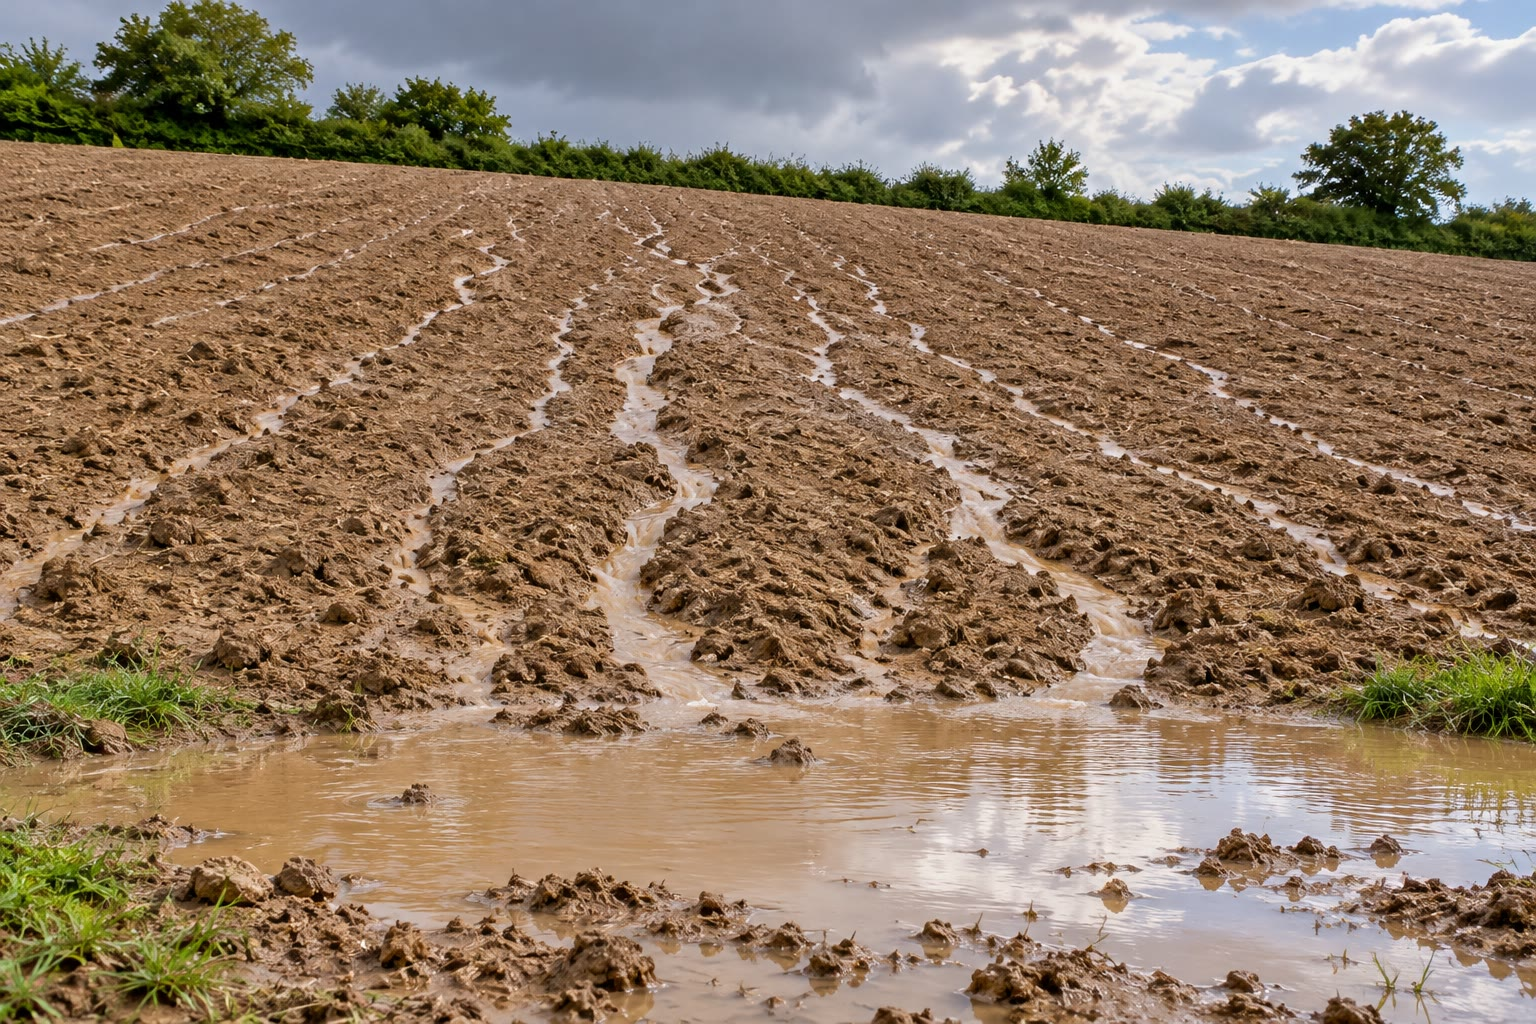
\includegraphics[width=0.72\linewidth]{images/book2/ai/g10-ploughed-rills.jpg}

{\small Ladang yang dibajak setelah hujan badai yang lebat: air larian telah
memotong saluran-saluran kecil, atau alur, menuruni lereng dan membawa tanah
ke dalam genangan berlumpur di kakinya.}
\end{omfigure}

\section{Latihan}

\begin{exercise}[$\star$]\label{exo:g10:soil-formation:1}
Definisikan \omterm{def:g10:soil-formation:chemical-weathering}{pelapukan kimia} dan \omterm{def:g10:soil-formation:hydrolysis}{hidrolisis}.
\end{exercise}

\begin{exercise}[$\star$]\label{exo:g10:soil-formation:2}
Apakah \omterm{def:g10:soil-formation:weathering-profile}{saprolit} itu? Bagaimana kamu dapat membedakan \omterm{def:g10:soil-formation:weathering-profile}{saprolit} dari tanah yang
terbentuk pada pasir yang dibawa sungai?
\end{exercise}

\begin{exercise}[$\star$]\label{exo:g10:soil-formation:3}
Sebutkan hasil-hasil pelapukan granit: menjadi apakah masing-masing dari tiga
mineral utamanya?
\end{exercise}

\begin{exercise}[$\star$]\label{exo:g10:soil-formation:4}
Mengapa batuan yang lapuk dan tanah tropis begitu sering berwarna merah, kuning, atau cokelat?
\end{exercise}

\begin{exercise}[$\star$]\label{exo:g10:soil-formation:5}
Dengan diagram batang, sebutkan laju median produksi tanah dan laju erosi
median di bawah pembajakan konvensional. Berapa kali lebih besar laju yang
kedua?
\end{exercise}

\begin{exercise}[$\star\star$]\label{exo:g10:soil-formation:6}
Periksalah bahwa persamaan pelarutan kalsit setara, untuk setiap unsur dan
untuk muatannya.
\end{exercise}

\begin{exercise}[$\star\star$]\label{exo:g10:soil-formation:7}
Batu kapur melarut sepenuhnya, granit meninggalkan pasir dan lempung.
Jelaskan perbedaannya dengan dua reaksi dalam bab ini.
\end{exercise}

\begin{exercise}[$\star\star$]\label{exo:g10:soil-formation:8}
Jelaskan bagaimana kompleks lempung--humus menahan kalium dalam tanah yang
tercuci oleh hujan, dan bagaimana akar mengambilnya.
\end{exercise}

\begin{exercise}[$\star\star$]\label{exo:g10:soil-formation:9}
Berikan dua alasan mengapa \omterm{def:g10:soil-formation:laterite}{laterit} terbentuk di bawah iklim panas dan basah,
dan tidak di bawah iklim dingin atau kering.
\end{exercise}

\begin{exercise}[$\star\star$]\label{exo:g10:soil-formation:10}
Laju median produksi tanah adalah \qty{0.017}{mm} setahun. Berapa lama waktu
yang diperlukan untuk membentuk \qty{1}{cm}, \qty{30}{cm}, dan \qty{1}{m}
tanah?
\end{exercise}

\begin{exercise}[$\star\star$]\label{exo:g10:soil-formation:11}
Laju erosi sering dinyatakan sebagai massa tanah per hektare per tahun.
Dengan massa jenis tanah \qty{1200}{kg/m^3}, berapa massa yang diwakili oleh
kehilangan \qty{1.5}{mm} setahun pada satu hektare (\qty{10000}{m^2})?
\end{exercise}

\begin{exercise}[$\star\star\star$]\label{exo:g10:soil-formation:12}
\omterm{def:g10:soil-formation:weathering-profile}{Saprolit} setebal \qty{46}{m} telah terbentuk di bawah perbukitan sebuah
daerah beriklim sedang. Jika pelapukan maju ke dalam batuan dengan laju
\qty{0.017}{mm} setahun, berapa lama waktu yang diperlukannya? Apa yang
diisyaratkan jawaban itu tentang umur bentang alam seperti itu?
\end{exercise}

\begin{exercise}[$\star\star\star$]\label{exo:g10:soil-formation:13}
Tuliskan persamaan oksidasi \ce{Fe^2+} menjadi goetit yang diberikan dalam bab
ini dan periksalah. Lalu tuliskan dan setarakan oksidasi \ce{Fe^2+} menjadi
hematit, \ce{Fe2O3}, oleh oksigen dan air, yang melepaskan \ce{H+}.
\end{exercise}

\begin{exercise}[$\star\star\star$]\label{exo:g10:soil-formation:14}
Di bawah pertanian konservasi laju erosi mediannya \qty{0.082}{mm} setahun.
Dengan produksi tanah \qty{0.017}{mm} setahun, berapa lama waktu yang
diperlukan untuk kehilangan \qty{30}{cm} tanah? Bandingkan dengan pembajakan
konvensional.
\end{exercise}

\begin{exercise}[$\star\star\star$]\label{exo:g10:soil-formation:15}
Sebuah granit mengandung \qty{30}{\percent} ortoklas menurut massa. Berapa
massa kaolinit yang terbentuk bila seluruh ortoklas dalam satu ton granit ini
telah melapuk, dan berapa massa kalium yang dilepaskan?
\end{exercise}

\section{Soal: Umur Sebuah Tanah}

\begin{problem}[{Soal akhir pekan --- dari batuan ke ladang dan kembali ke sungai}]
\label{pb:g10:soil-formation:1}
% ledger: montgomery:rates, montgomery:lifetime, webmineral:formulas (values computed in figdata/grade-10/soil_rates.py)

\begin{center}
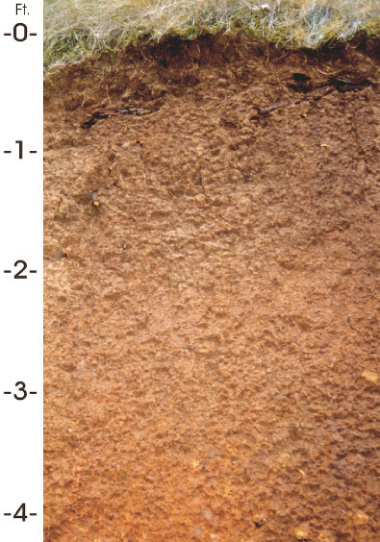
\includegraphics[height=6cm]{images/book2/g10-nrcs-jory-soil.jpg}

{\small Sebuah profil tanah, dengan skala dalam kaki di sebelah kiri (\num{1}~kaki =
\qty{0.3048}{m}). Foto: USDA Natural Resources Conservation Service
(domain publik).}
\end{center}

\medskip
\noindent\textbf{Bagian I --- Sebuah profil.}
\begin{enumerate}
  \item Skala itu mencapai 4 kaki di dekat bagian bawah gambar. Berapa
        dalamnya itu, dalam meter?
  \item Lapisan gelap di bagian atas mencapai sekitar setengah kaki. Berapa
        tebalnya, dalam sentimeter?
  \item Apa yang memberi lapisan atas ini warna gelapnya?
  \item Di bawahnya, tanah berwarna cokelat kemerahan. Mineral apa yang
        memberinya warna ini, dan bagaimana mineral itu terbentuk?
  \item Apakah \omterm{def:g10:soil-formation:weathering-profile}{batuan induk} terlihat pada foto itu? Apa yang akan kamu
        harapkan ada di bawah bagian bawah gambar?
\end{enumerate}

\medskip
\noindent\textbf{Bagian II --- Kimia granit yang sedang melapuk.}
\begin{enumerate}[resume]
  \item Tuliskan persamaan \omterm{def:g10:soil-formation:hydrolysis}{hidrolisis} ortoklas.
  \item Berapa mol ortoklas yang ada dalam \qty{1}{kg}
        (\qty{278.33}{g/mol})?
  \item Berapa massa kaolinit (\qty{258.16}{g/mol}) yang dihasilkannya?
  \item Apa yang pergi bersama air, dan ke mana perginya?
  \item Apa yang terjadi pada kuarsa granit itu?
\end{enumerate}

\medskip
\noindent\textbf{Bagian III --- Pembentukan melawan erosi.}
\begin{enumerate}[resume]
  \item Tanah terbentuk dengan laju \qty{0.017}{mm} setahun. Berapa lama
        waktu yang diperlukan untuk membentuk profil pada Bagian I?
  \item Di bawah pembajakan konvensional, tanah tererosi dengan laju
        \qty{1.537}{mm} setahun. Berapa kehilangan bersih setiap tahun?
  \item Berapa lama profil pada Bagian I akan bertahan?
  \item Bandingkan kedua waktu pada pertanyaan 11 dan 13.
  \item Di bawah vegetasi alami, erosi \qty{0.013}{mm} setahun. Apakah tanah
        itu sedang hilang?
\end{enumerate}

\medskip
\noindent\textbf{Bagian IV --- Umur tanah.}
\begin{enumerate}[resume]
  \item Tuliskan waktu $T$ untuk kehilangan tanah setebal $S$ sebagai fungsi
        dari $S$, laju erosi $E$, dan laju produksi $P$.
  \item Hitung $T$ untuk $S = \qty{30}{cm}$ di bawah pembajakan
        konvensional.
  \item Hitung $T$ untuk $S = \qty{30}{cm}$ di bawah pertanian konservasi
        (\qty{0.082}{mm} setahun).
  \item Mengapa tanah dapat disebut sumber daya yang tidak terbarukan pada
        skala waktu manusia?
  \item Berapa lama waktu yang diperlukan untuk kehilangan satu meter tanah di
        bawah pembajakan konvensional?
\end{enumerate}
\end{problem}
